\section{Effective forces on nanomolecular scales}
\label{appendix:nanomolecular}

In classical mechanics an object moving in fluid is affected by forces: weight (directed down), buoyant force (directed up), drag force (directed opposite the direction of movement). During capsid disassembly there are also forces exerted by molecular motors and restoring forces of bonds between M1.

\begin{center}
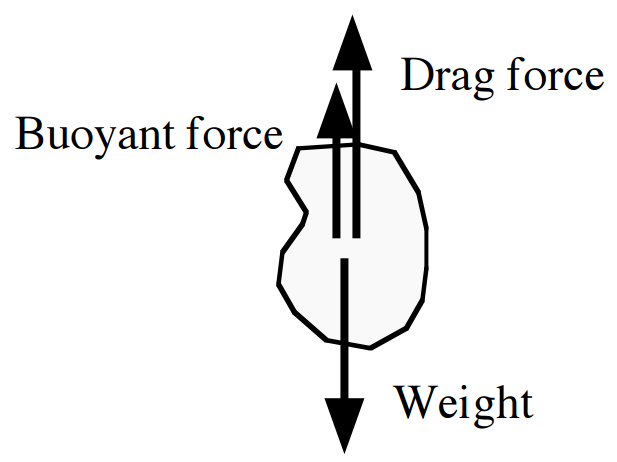
\includegraphics[width=0.5\textwidth]{D_chapters/1_TugOfWar/Sedimentation.PNG}
\captionof{figure}{Forces affecting object during sedimentation in fluid.}
\end{center}

The Reynolds number is the ratio of inertial forces to viscous forces within a fluid which is subjected to relative internal movement due to different fluid velocities. In systems with low Reynolds numbers it's sometimes possible to omit inertial forces as fluid dynamic play a much more important role \cite{purcell1977life}.

Let's estimate sedimentation forces and mechanical forces involved in capsid disassembly, to determine their relevancy to mathematical modelling.

\subsection{Reynolds number}

Reynolds number is defined as

\begin{equation}
Re = \frac{\text{inertial forces}}{\text{viscous forces}} =\frac{av\rho}{\eta} = \frac{av}{\nu}
\end{equation}

where $a$ is a characteristic size of the moving object, $v$ is its velocity relative to fluid, $\rho$ is fluid density, $\eta$ is fluid viscosity and $\nu$ is kinematic viscosity.

\begin{center}
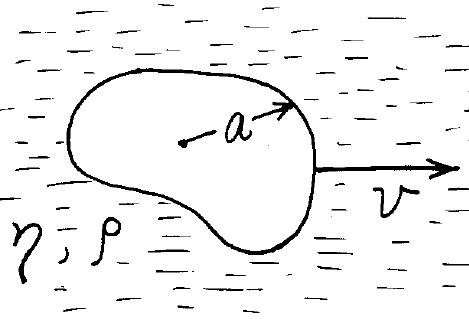
\includegraphics[width=0.5\textwidth]{D_chapters/1_TugOfWar/Reynolds_number.PNG}
\captionof{figure}{Object of characteristic size $a$ moving with speed $v$ in fluid with density $\rho$ and viscosity $\eta$.}
\end{center}

Let's calculate Reynolds number for influenza A capsid protein M1.

M1 characteristic size $a = 4 \text{ nm} = 4 \cdot 10^{-7} \text{ cm}$ \cite{shtykova2013structural}.

During calculation individual velocities of the nodes typically are in the range of $10^{-13}$-$10^{-5} \text{ m/s}$. Motor forward velocities are around $10^{-6} \text{ m/s}$ \cite{muller2008tug}. Let's assume for this calculation that $v = 10^{-6} \text{ m/s} = 10^{-4} \text{ cm/s}$.

Average density of the cytoplasm (horn cells in rats, only available data?) is about $\rho = 0.3 \text{ pg}/\SI{}{\micro\meter}^3 = 0.3 \text{ g}/\text{cm}^3$ \cite{hartmann1967cytoplasmic}. Alternatively (\textit{E. coli}) $\rho = 1.1 \text{ g}/\text{cm}^3$ \cite{loferer1998determination}.

Relative viscosity of cytoplasm (cytoplasm versus water) determined by time-resolved microfluorimetry \cite{swaminathan1997photobleaching} is

\begin{equation}
\frac{\eta_\text{cytoplasm}}{\eta_\text{water}} = 1.5,
\end{equation}

and determined by photobleaching recovery of green fluorescent protein \cite{swaminathan1997photobleaching} is 

\begin{equation}
\frac{\eta_\text{cytoplasm}}{\eta_\text{water} }= 3.2.
\end{equation}

Water viscosity is $\eta_\text{water} = 8.9 \cdot 10^{-3} \text{ dyn} \cdot \text{s}/\text{cm}^2 = 8.9 \cdot 10^{-3} \text{ g}/\text{cm} \cdot \text{s} $ at \SI{25}{\degreeCelsius} \cite{IAPWS2008}. So $\eta_\text{cytoplasm} = 3.2 \cdot 8.9 \cdot 10^{-3} \text{ g}/(\text{cm} \cdot \text{s}) = 28.5 \cdot 10^{-3} \text{ g}/(\text{cm} \cdot \text{s})$.

Thus, Reynolds number is

\begin{equation}
Re = \frac{av\rho}{\eta} = \frac{4 \cdot 10^{-7} \text{ cm} \cdot 10^{-4} \text{ cm/s} \cdot 0.3 \text{ g}/\text{cm}^3}{28.5 \cdot 10^{-3} \text{ g}/(\text{cm} \cdot \text{s})} = 4.2 \cdot 10^{-10}
\end{equation}

This value is extremely small - for comparison, the Reynolds number for a bacteria moving in the medium is (?)

\subsection{Weight}

\begin{equation}
F_{\text{weight}} = mg,
\end{equation}

where $m$ is object mass and $g$ is gravitational acceleration.

The mass of M1 capsid protein is $m_{\text{M1}} = 28 \text{ kDa} = 28 \cdot 1000 \cdot 1.66 \cdot 10^{-27} \text{ kg} = 46.5 \cdot 10^{-24} \text{ kg}$. \cite{shtykova2013structural}

Then the force is

\begin{equation}
F_{\text{weight}} = m_{M1}g = 46.5 \cdot 10^{-24} \text{ kg} \cdot 9.8 \text{ m}/\text{s}^2 = 4.6 \cdot 10^{-22} \text{ N}
\end{equation}

\subsection{Buoyant force}

\begin{equation}
F_{\text{buoyant}} = \rho_FVg,
\end{equation}

where $\rho_F$ is density of the fluid, $V$ is the volume of the object and $g$ is gravitational acceleration.

Density of cytoplasm as previously established is $\rho = 0.3 \text{ g}/\text{cm}^3 = 3000 \text{ kg}/\text{m}^3$ \cite{hartmann1967cytoplasmic}

Dimensions of M1 protein are approximately $4.0 \times 4.0 \times 6.0 \text{ nm}$ \cite{shtykova2013structural}, so $V_{M1} = 96 \text{ nm}^3 = 9.6 \cdot 10^{-26} \text{ m}^3$

Then the force is

\begin{equation}
\begin{split}
F_{\text{buoyant}} = \rho_{\text{cytoplasm}}V_{M1}g =\\
3000 \text{ kg}/\text{m}^3 \cdot 9.6 \cdot 10^{-26} \text{ m}^3 \cdot 9.8 \text{ m}/\text{s}^2 =\\
2.8 \cdot 10^{-21} \text{ N}
\end{split}
\end{equation}

\subsection{Drag force}

Drag force exerted on spherical objects with very small Reynolds numbers (i.e. very small particles) in a viscous fluid is defined by Stokes' law:

\begin{equation}
F_{\text{drag}} = 6\pi\eta av,
\end{equation}

where $\eta$ is dynamic fluid viscosity, $a$ is the radius of the spherical object, $v$ is the flow velocity relative to the object.

As previously shown $\eta_{\text{cytoplasm}} = 28.5 \cdot 10^{-3} \text{ g}/(\text{cm} \cdot \text{s}) = 2.85 \cdot 10^{-4} \text{ kg}/(\text{m} \cdot \text{s})$ \cite{swaminathan1997photobleaching, IAPWS2008}.

M1 characteristic size $a = 4 \text{ nm} = 4 \cdot 10^{-9} \text{ m}$ \cite{shtykova2013structural}.

And velocities are in range $v = 10^{-6} \text{ m/s}$ \cite{muller2008tug}.

Then the force is

\begin{equation}
\begin{split}
F_{\text{drag}} = 6\pi\eta_{\text{cytoplasm}} av = \\
6 \cdot 3.14 \cdot 2.85 \cdot 10^{-4} \text{ kg}/(\text{m} \cdot \text{s}) \cdot 4 \cdot 10^{-9} \text{ m} \cdot 10^{-6} \text{ m/s} =\\
2.1 \cdot 10^{-17} \text{ N}.
\end{split}
\end{equation}

\begin{center}
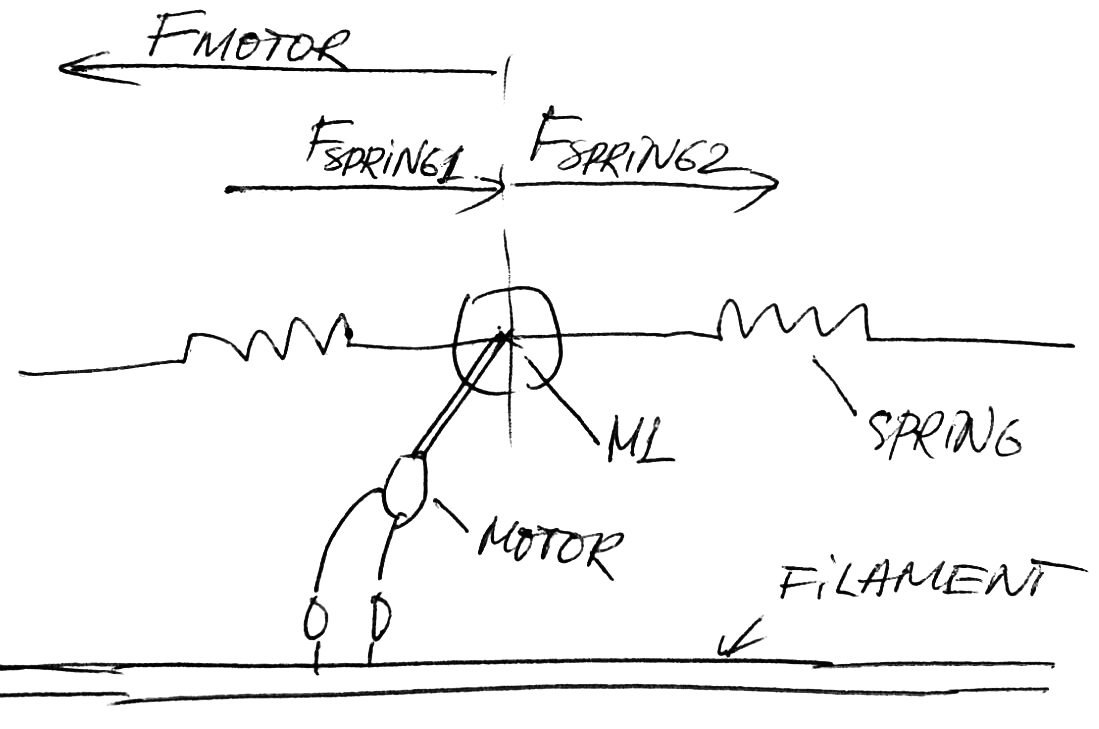
\includegraphics[width=0.5\textwidth]{D_chapters/1_TugOfWar/Capsid.jpg}
\captionof{figure}{Forces affecting M1 capsid protein during capsid disassembly.}
\end{center}

\subsection{Motor forces}

Stall forces of molecular motors are in orders of pN \cite{muller2008tug}, which leads to resulting tug-of-war forces to be of the same order $F_{\text{motor}} = 10^{-12} \text{ N}$.

\subsection{Spring forces}

In the simplest case spring forces can be calculated using Hooke's law:

\begin{equation}
F_{\text{Hooke}} = k_{\text{spring}}\Delta x.
\end{equation}

At pH of interest the bond spring constant is $k_{\text{spring}} = 2.1 \cdot 10^{-2} \text{ N}/\text{m}$ \cite{li2014ph}

The displacements in the calculation are of the order of the equilibrium length of the spring: $\Delta x = 4 \text{ nm} = 4 \cdot 10^{-9} \text{ m}$

Then the force is

\begin{equation}
\begin{split}
F_{\text{Hooke}} = k_{\text{spring}}\Delta x =\\
2.1 \cdot 10^{-2} \text{ N}/\text{m} \cdot 4 \cdot 10^{-9} \text{ m} = 8.4 \cdot 10^{-11} \text{ N}.
\end{split}
\end{equation}

In our representation of capsid disassembly instead of Hooke's law we're using Morse potential, because it explicitly includes the possibility of break:

\begin{equation}
V(\mathbf{r}) = D_{\text{e}} \big(1 - e^{- a(\mathbf{r - r_e})}\big)^2 = D_{\text{e}} \big(1 - e^{- a \Delta \mathbf{r}}\big)^2.
\end{equation}

Here $\mathbf{r}$ is the distance, $\mathbf{r_e}$ is the equilibrium bond distance, $D_{\text{e}}$ is the well depth,

\begin{equation}
a=\sqrt {\frac{k_{\text{e}}}{2D_{\text{e}}}},
\end{equation}

where $k_e$ is the force constant at the minimum of the well. $a$ controls the ``width'' of the potential (the smaller $a$ is, the larger the well).

The restoring force is

\begin{equation}
\mathbf{F}_\text{Morse} = - 2a D_{\text{e}}e^{- a |\Delta \mathbf{x}|}\big(1 - e^{- a |\Delta \mathbf{x}|}\big) \cdot \big(- \frac{\Delta \mathbf{x}}{|\Delta \mathbf{x}|}\big).
\end{equation}

For $D_{\text{e}} = 20 \text{kJ}$ (the energy of hydrogen bond \cite{mcnaught1997compendium}) and $k_{\text{e}} = k_{\text{spring}} = 2.1 \cdot 10^{-2} \text{ N}/\text{m}$

\begin{equation}
\begin{split}
a = \sqrt {\frac{2.1 \cdot 10^{-2} \text{ N}/\text{m}}{2 \cdot 2 \cdot 10^{4} \text{J}}}\\
= \sqrt {\frac{2.1 \cdot 10^{-2} (\text{ kg} \cdot \text{m} \cdot \text{s}^-2)/\text{m}}{2 \cdot 2 \cdot 10^{4} (\text{ kg} \cdot \text{m}^2 \cdot \text{s}^-2)}} = 7.2 \text{ m}^{-1}
\end{split}
\end{equation}

\begin{equation}
e^{- a |\Delta \mathbf{x}|} = e^{- 7.2 \text{ m}^{-1} \cdot 4 \cdot 10^{-9} \text{ m}} = 1
\end{equation}

\begin{equation}
1 - e^{- a |\Delta \mathbf{x}|} = 1 - e^{- 7.2 \text{ m}^{-1} \cdot 4 \cdot 10^{-9} \text{ m}} = 2.9 \cdot 10^{-9}
\end{equation}

\begin{equation}
\begin{split}
F_\text{Morse} = 2aD_{\text{e}}e^{- a |\Delta \mathbf{x}|}\big(1 - e^{- a |\Delta \mathbf{x}|}\big) =\\
2 \cdot 7.2 \text{ m}^{-1} \cdot 2 \cdot 10^{4} \text{J} \cdot 1 \cdot 2.9 \cdot 10^{-9} = 8.4 \cdot 10^{-4} \text{ N}.
\end{split}
\end{equation}

On first calculation steps these forces are about $10^{-21} \text{ N}$ but reach up to $10^{-9} \text{ N}$ during the course of the calculation.

\subsection{Conclusion}

In our model we can only focus on spring and motor forces as sedimentation forces acting on the proteins are negligibly small.

